% Chapter Template

\chapter{Related work} % Main chapter title


\label{ChapterX} % Change X to a consecutive number; for referencing this chapter elsewhere, use \ref{ChapterX}

The state of the art related to this particular project is classified on four different types of solutions that focus on giving developers tools to test their web applications on different kinds of platforms: Proprietary solutions, crowd sourced testing, open source software and scientific research.

%----------------------------------------------------------------------------------------
%	SECTION 1
%----------------------------------------------------------------------------------------

\section{Proprietary Solutions}

This is a niche of solutions for testing fragmentation on web applications: BrowserStack, SouceLabs, LambdaTest, Browserling, CrossBrowserTesting, just to name a few. Coming up, we will expose some of them that offer a free trial to test what they can offer.

\subsection{BrowserStack}
TODO: Fill out with content from proposal

\subsection{LambdaTest}
TODO: Fill out with content from proposal

\section{Crowd sourced testing}
Crowd sourced testing consists on distributing an application for testing on different machines and pay those who are willing to execute tests for such software. Although it is common in other types of software like games and mobile apps, it is not viable for web, since it requires a high costs compared to automation tools. 
Besides, it does not have the possibility to scale so easily as automated tests do. Meaning, one round of crowd sourced testing covers a specific version of the software; in order to test another version with corrections, other round is required, which is time and money consuming. Since web applications change constantly, this option becomes non-practical on the real life. 

\section{Open Source Software}

\subsection{Galen}

TODO: Fill out with information

\subsection{BackstopJS}

TODO: Fill out with information

\section{Scientific Research}

Taking a look into the literature, there are two main methods that offer developers the opportunity to know how their application looks in different browsers: Visual regression testing and runtime code analysis. 

\subsection{Visual regression testing}

It consists in generating images that show the places or actions where the same application is different when compared to a different browser. Alongside this line of research you can find tools like WEBDIFF and CrossCheck.

\textbf{WEBDIFF.} The main idea is to collect information from the DOM of each browser and capture a screenshot of the web page at a given time. Then. having a reference browser, mark all elements that vary when compared to such DOM. Finally, compare the information using the images and generate a list of elements that are different. 

\textbf{CrossCheck.} Use of the best of two different tools: Webdiff (Already explained above) and CROSST. Meanwhile Webdiff is very useful for detecting XBIs related to how the screen looks in different browsers, CROSST is used for finding trace-level XBIs. When talking about trace-level, we refer to detection of differences on the elements of the DOM by performing a static code check. In top of this, Crosscheck introduces machine learning to build a classifier for visual comparison of elements. 





As part of the problem definition, we reviewed previous papers focused on static analysis of android apps at APK level, with the purpose of identifying the intermediate representations used by researchers. Therefore, we queried publications with  the keywords: "smali code", "smali", "APK processing", "android apk" and "apk files", "android Smali". Most of the retrieved works focused mainly on security. As part of the results we found a paper called "Static Analysis of Android Apps A Systematic Literature Review" \cite{li:IaST2017} wrote by Li \textit{et. al.} Therefore, instead of conducting a new mapping study or literature review by ourselves, we relied on the work by Li \textit{et. al.}.

The paper Li \textit{et. al.}, in the authors words, \textit{``provide a clear view of the state-of-the-art works that statically analyze Android apps, from which we [the authors] highlight the trends of static analysis approaches, pinpoint where the focus has been put, and enumerate the key aspects where future researchers are still needed''}. In particular, Li \textit{et. al.,} conducted a systematic literature review using the search string shown in Table \ref{table:liss}, which reports 124 papers and classifies them in 8 categories depicted in Figure \ref{fig:sAPD}: (i) Private Data Leaks (46 papers), (ii) Vulnerabilities (40 papers), (iii) Permission Misuse (15 papers), (iv) Energy Consumption (9 papers), (v) Clone Detection (7 papers), (vi) Test Case Generation (6 papers), (vii) Cryptography Implementation Issues (3 papers) and (vii) Code verification (3 papers). 

Note that the systematic literature review by Li \textit{et. al.,} considers only papers up to 2015, and we recognize that since then several works could have been published. Our purpose with reviewing previous papers was to identify the existing intermediate representations and their characteristics. Therefore, not having a complete literature review until 2018 is not a limitation for our work.   Future work, should be devoted to conduct a more up-to-date literature review that also includes previous papers that use dynamic analysis.

In the following, we briefly describe the task-related groups used by Li \textit{et. al.,} and discuss some of the representative papers.
\begin{table}[t]
	\centering
		\caption{Keywords used by Li \textit{et. al.}}
	\label{table:liss}
	\begin{tabular}{|p{1cm} | p{10cm}|} 
		\hline
		Line & Keywords \\ [0.5ex] 
		\hline\hline
		1 & Analisis; Analyz*; Analys*; \\ 
		2 & Data-Flow; "Data Flow*"; Control-Flow; "Control Flow"; "Information-Flow*"; "Information Flow*"; Static*; Taint; \\
		3 & Android; Mobile; Smartphone*; "Smart Phone"; \\
		\hline
	\end{tabular}

\end{table}

\begin{figure}[t]
\caption{Statistics of main concerns addressed by the publications presented in Li \textit{et. al.} publication}
\centering
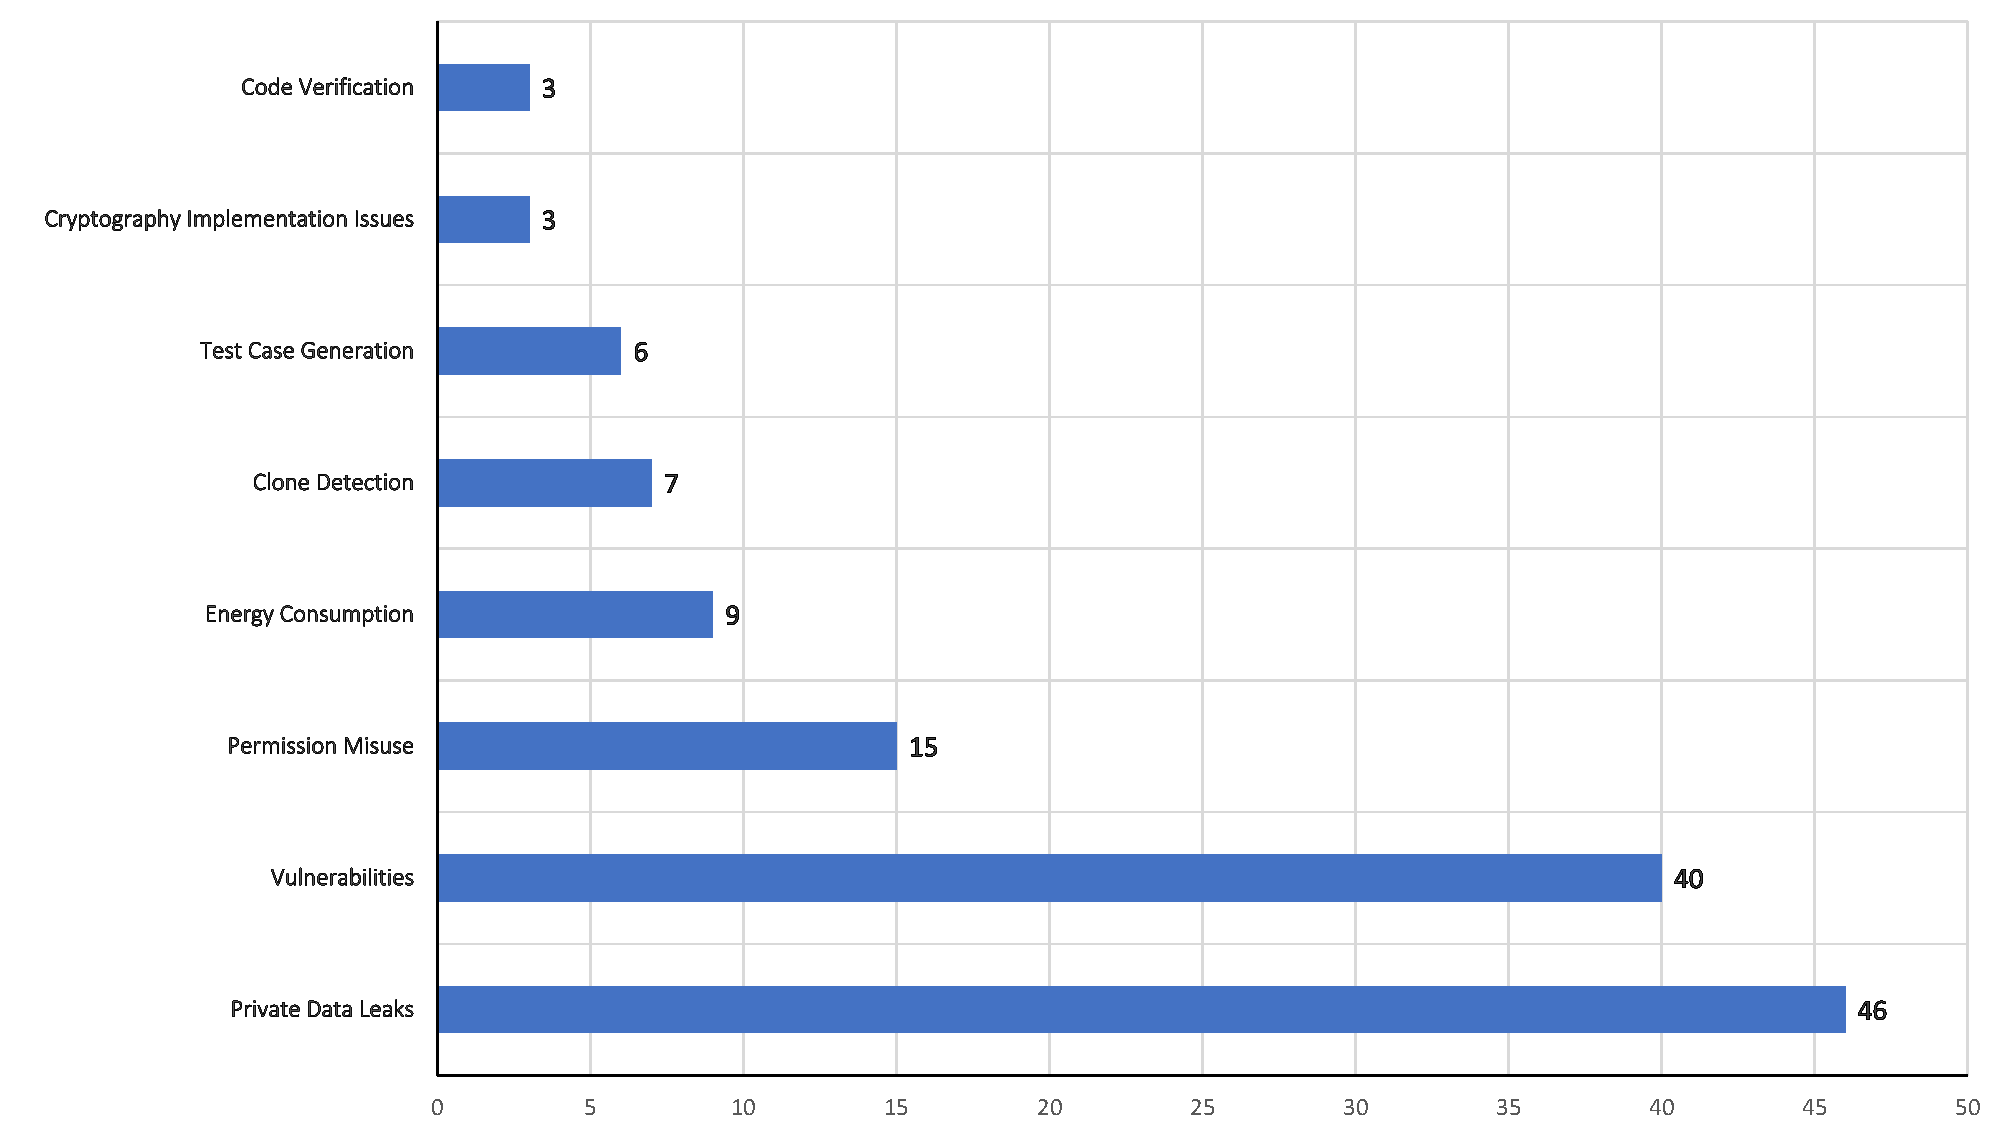
\includegraphics[width=\textwidth]{../Figures/publicationDistribution}
\label{fig:sAPD}
\end{figure}



\textbf{Private Data Leaks.} This is the most frequent purpose reported in the papers categorized by Li \textit{et. al.,}. In this group, FlowDroid is a representative example \cite{Arzt:2014}; FlowDroid  performs static taint analysis on android apps using flow-, context-, field-, object-sensitive and implicit flow-, lifecycle-, static-, alias-aware analysis. Therefore, FlowDroid has became a defacto tool used by researchers interested on finding privacy leaks in Android apps. For example, PCLeaks \cite{li:TrustCom2014} goes one step further by performing sensitive data-flow analysis on top of component vulnerabilities, enabling not only issue identification but also data endangered. The most used intermediate representation for this category of papers is JIMPLE with 18 out of 46 papers, followed by SMALI with 8 papers.

\textbf{Vulnerabilities.} This category groups papers aiming at detecting vulnerabilities in Android apps. For instance,  CHEX\cite{lu:CCS2012} that detects potential component hijacking-based flows through reachability analysis on customized system dependence graphs and, Epicc \cite{octeau:Security2013} and IC3 \cite{octeau:ICSE2015} that implement static analysis techniques for implementing detection scenarios of inter-component vulnerabilities. The most used intermediate representation for this category of papers is SMALI with 15 out of 40 papers, followed by JIMPLE with 6 papers.

\textbf{Permission Misuse.} Permissions are one of the core elements of the Android security model. Malware applications try to use the permissions granted by the user to perform actions that do not correspond to the app features. Lin \textit{et. al.} \cite{lin2014modeling} conducted an study of  permissions that users are most comfortable to grant, creating a set of privacy profiles, and in which way applications use those permissions. The most used intermediate representation for this category of papers is JIMPLE with 6 out of 15 papers, followed by SMALI with 4.

\textbf{Energy Consumption}.  APIs and some hardware components have been demostrated as energy greedy elements in Android apps \cite{Linares-Vasquez:2014,Pathak:2011}, thus, analysis of energy consumption of mobile apps is becoming a hot topic. For instance, Li \textit{et. al.} \cite{li:ISSTA2013} present a tool to calculate source line level energy consumption through combining program analysis and statical modeling. The output of these analyses can then be leveraged to perform quantitative and qualitative empirical investigations into the categories of API calls and usage patterns that exhibit energy consumptions profiles. The most used intermediate representation for this category of papers is JAVA\_CLASS with 6 out of 9 papers, followed by JIMPLE with 2.

\textbf{Clone Detection.} It is also well known that there are some circumstances that lead app users to use APK repositories different from Google Play, which generates a concern about the origin and provenance of Android apps in general. Therefore, approaches such as DNADroid\cite{crussell:ESORICS2012} uses neural networks and dinamic-, static analysis to propose detection of ransomware before infection happens. At the same time, Crusell \textit{et. al.,} \cite{crussell:ESORICS2013} propose a scalable to detecting similar Android Apps based on their semantic information. The most used intermediate representation for this category of papers is SMALI with 3 out of 7 papers, followed by DEX\_ASSEMBLER with 2.

\textbf{Test Case Generation.} A common way to perform analysis of an application is using systematic exploration, nevertheless running real world applications in real devices is cumbersome due to several problems like non-determinism, non-standard control flow, etc. Because of this, A3E\cite{azim:OOPSLA2013} uses static, taint-style, dataflow analysis on the app bytecode to construct a higher level flow-graph that captures legal transition among activities, and can be used to explore the app in a user-like behavior. At the same time, Jensen \textit{et al.}\cite{jensen:ISSTA2013} propose a two-phase technique that uses concolic execution to build summaries of the event handlers of the application and builds event sequences backward from the target, enabling the testing of parts that require more complex event sequences. The most used intermediate representation for this category of papers is JIMPLE with 3 out of 6 papers, followed by WALA\_IR and SMALI with 1 paper each one.

\textbf{Code Verification.} 
Code verification intends to ensure the correctness of a given app but without testing (\textit{i.e.,} app execution). For instance, Cassandra \cite{lortz:SPSMD2014} is proposed to check whether Android apps comply with their personal privacy requirements before installing an app. As another example, researchers have also extended the Julia \cite{payet:IST2012} static analyzer to perform code verification through formal analyses of Android programs. The most used intermediate representation for this category is JAVA\_CLASS with 2 papers.

\textbf{Cryptography Implementation Issues.} In addition to the aforementioned concerns, state-of-the-art works have also targeted cryptography implementation issues. As an example, CMA \cite{shuai2014modelling} performs static analysis on Android apps and select the branches that invoke the cryptographic API. Then it runs the app following the target branch and records the cryptographic API calls. At last, the CMA identifies the cryptographic API misuse vulnerabilities from the records based on the pre-defined model.
It is worth noticing that the top representations used by the reported papers are JIMPLE (38 papers), SMALI (26 papers) and JAVA\_CLASS (22 papers), and the main concern covered is security with around 101 papers.

\begin{figure}[h!]
	\caption{Intermediate representation distribution(i.e., number of papers) vs. purpose of the analysis}
	\centering
	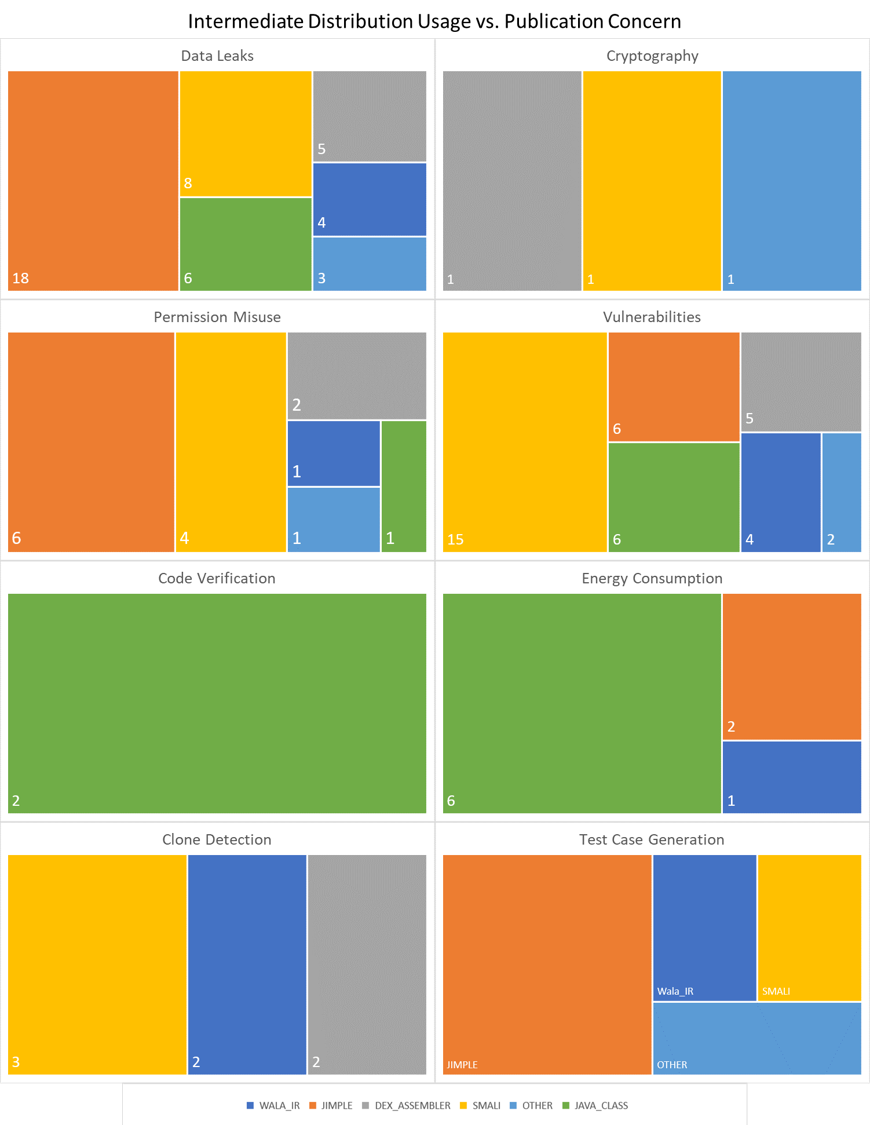
\includegraphics[width=\textwidth]{../Figures/IRvsPC}
	\label{fig:irvspc}
\end{figure}

Therefore, as we wanted to use an intermediate representation that is closer to the compiled code, we have to choose between JIMPLE and SMALI. Because of this, we extended our research to find existing studies aimed at comparing these two intermediate representations. After a short review in google scholar, we found a paper  by Arnatovich \textit{et. al.,}\cite{arnatovich2014empirical} called \textit{Empirical Comparison of Intermediate Representations for Android Applications} in which they study the preserveness of program behavior, by \textit{disassembling, assembling, signing, aligning and installing} 520 applications selected from the Google Play Store. The way they studied this was by running a random GUI-based input generation program (\textit{i.e., monkey runner}) over each app before and after the designed process\footnote{The monkey runner generates a seed that when given as parameter replicates the same events.} and collecting the amount of apps that crashed. Using this result, they were able to identify the amount of apps that do not crash after this process. The results of the study are summarized in Table \ref{tab:cpbp}:

\begin{table}[h!]
	\centering
	\caption{Comparision of program behavior preserveness for SMALI, JIMPLE and JASMIN}
	\label{tab:cpbp}
	\begin{tabular}{|C{3cm}|C{5cm}|}
		\hline
		Intermediate Representation& Preserved Program Behaviors of Original Applications (\%) \\
		\hline \hline
		SMALI&97.68\\
		JIMPLE&85.58\\
		JASMIN&81.92\\
		\hline
	\end{tabular}
\end{table}

Therefore, knowing that SMALI is the intermediate representation that preserves more the program behavior, we decided to use it along with the tool studied to generate mutants that only get affected by the mutation process.

\section{Mutation Testing for Android Apps} \label{sec:MT}

There are some previous work devoted to Mutation testing for Android apps. First, Linares-V\'asquez \textit{et. al.,}\cite{linares2017enabling,Moran:ICSE18} (to the best of our knowledge) have implemented the most comprehensive tool for mutation testing at source code level, MDroid+. They empirically extracted a taxonomy of crashes/bugs in android apps, and based on that, then proposed a set of 38 mutation operators. At the same time, Deng \textit{et al., } \cite{deng2015towards}, presented a set of eight mutant operators oriented to mutate core components of android (\textit{e.g., intents, event handlers, XML files and activity lifecycle}). Deng \textit{et al.} ,presented in 2017 the implementation of their 8 mutation operators in their paper "Mutation Operators for Testing Android Apps"\cite{deng2017mutation}. Finally, the last work found was muDroid\cite{mudroid} a mutation testing tool that works at APK level, but it implements standard mutation operators. However, MDroid+ authors \cite{linares2017enabling,Moran:ICSE18}  found that muDroid generates around 53\% of non-compilable mutants, that can be translated into a lost of half of the time invested on executing muDroid.

